%---------------------------------------
\section{INTRODUCCIÓN} \label{sec:Introduccion}
%---------------------------------------
El presente documento pretender exponer las dificultades algebraicas que plantea el cálculo de la velocidad de avance generada a través del movimiento de onda viajera realizado por microorganismos \cite{Gray1955} y animales acuáticos (peces \textit{Carangiform}) \cite{Korkmaz2012,Korkmaz2011}. Exponer una solución a estas dificultades mediante computación numérica e interpretar y analizar los resultados ofrecidos por la solución propuesta.\\

El movimiento de onda viajera realizado por la mayoría de los peces, según la ictiología es doblando su cuerpo \cite{modeswim}. Este tipo de movimiento denominado \textit{``body and caudal fin''} (BCF) se encuentra categorizado en diferentes clases, de las cuáles el tipo \textit{Carangiform}  presenta la mayor similitud con el flagelo de las células. El movimiento descrito por este tipo de peces fue sugerido originalmente por Lighthill \cite{FLM:368244}, y su expresión matemática es
\begin{eqnarray}
	\label{eq:fish_traveling_wave}
	y (x,t) = (c_1 x + c_2 x^2) \sin \left( \frac{2 \pi}{\lambda}  ( x - V_p t) \right),
\end{eqnarray}
donde $x$ es el desplazamiento sobre el eje principal, $V_p$ la velocidad de propagación de las ondas respecto al cuerpo y de sentido contrario a la velocidad de avance, $\lambda$ la longitud de onda y $c_1$ y $c_2$ los coeficientes lineal y cuadrático de la amplitud de la onda, respectivamente. Esta expresión recoge la dinámica del movimiento \textit{Carangiform} realizado desde el punto de unión del cuerpo hasta el extremo final de la cola \cite{Robotic_Fish,Robotic_Fish_speed,Robotic_Fish_3D}. Para recoger en una misma expresión la posibilidad de una onda viajera armónica como la estudiada para los flagelos en \cite{gray1955propulsion}, se debe introducir un nuevo coeficiente $c_0$ quedando la expresión anterior de la forma
\begin{eqnarray}
	\label{eq:flag_fish_traveling_wave}
	y (x,t) = (c_0+c_1 x + c_2 x^2) \sin \left( \frac{2 \pi}{\lambda}  ( x - V_p t) \right).
\end{eqnarray}

En (\ref{eq:flag_fish_traveling_wave}), el coeficiente $c_0$ permite definir el movimiento armónico puro de la onda viajera, como se ilustra en la Figura \ref{fig:FC}, pero no define el realizado por la cola de un pez. Es necesario sustituirlo por el coeficiente $c_1$, que impone la condición de contorno $y(0,t) = 0$, es decir, el inicio de la cola se encuentra unido a la cabeza en todo instante de tiempo. Sin embargo, dicho coeficiente define una onda viajera cuya amplitud crece linealmente en el eje principal (ver Figura \ref{fig:FC}). Para corregir este comportamiento se introduce el término cuadrático $c_2$, con el cual es posible modular el crecimiento de la onda viajera para alcanzar una amplitud mantenida sobre el eje principal.
\begin{figure}[!h] %  figure placement: here, top, bottom, or page
	\vspace*{3mm}
    \centering
    \includegraphics[width=0.43\textwidth]{Figuras/FC}
  	\caption{Comparación de la onda viajera para diferentes coeficientes.}
  	\label{fig:FC}
\end{figure}

Siguiendo el análisis descrito en \cite{gray1955propulsion}, se puede extraer la velocidad de avance para el movimiento indicado en (\ref{eq:flag_fish_traveling_wave}) como:
\begin{eqnarray}
\label{eq:Vx_fish}
\begin{split}
	V_x (t)  =  \pi f\left( \frac{C_N - C_L}{C_L} \right) \left( \frac{1}{ 1 + \frac{6 \pi R \mu}{n \lambda C_L} }  \right)\\
(- \frac{2 \pi}{\lambda} c_0^2 - 2 \pi c_0 c_1 - \frac{4 \pi c_0 c_2}{3} \\ 
+ c_0 c_1 \sin \left( 4 \pi f t \right) + c_0 c_2 \sin \left( 4 \pi f t \right) - \frac{2 \pi \lambda}{3} c_1^2 \\
- \pi \lambda^2 c_1 c_2 + \frac{\lambda c_1^2}{2} \sin \left( 4 \pi f t \right) + \lambda^2 c_1 c_2 \sin \left( 4 \pi f t \right) \\
- \frac{2 \pi \lambda^3}{5} c_2^2 + \frac{\lambda^3 c_2^2}{2} \sin \left( 4 \pi f t \right) )
	 		\end{split}
\end{eqnarray}
donde se aprecia la influencia de los coeficientes para lograr diferentes magnitudes de velocidad, y la relación entre ellos. Esto implica una cierta dificultad para alcanzar una velocidad óptima, y mantener un movimiento de onda viajera cuyas oscilaciones sean moduladas y mantenidas (constantes) en el espacio.\\

Para simplificar este cometido se opta por una descripción diferente del movimiento de onda viajera descrito en (\ref{eq:flag_fish_traveling_wave}), basado en un coeficiente fraccionario que influye en la amplitud de la onda viajera en base a su ubicación en el espacio, siendo por lo tanto la nueva expresión de la forma
\begin{eqnarray}
	\label{eq:flag_fish_traveling_wave_fractional}
	y (x,t) = c_1 x^{\alpha} \sin \left( \frac{2 \pi}{\lambda}  ( x - V_p t) \right).
\end{eqnarray}
\

Esta nueva descripción permite determinar la amplitud máxima de las oscilaciones a partir del coeficiente $c_1$, y modular su crecimiento con el parámetro $\alpha$. La Figura \ref{fig:OVF} evidencia este comportamiento, donde se puede observar el crecimiento en amplitud de la onda para diferentes valores del parámetro $\alpha$.
\begin{figure}[!h] %  figure placement: here, top, bottom, or page
	\vspace*{3mm}
    \centering
    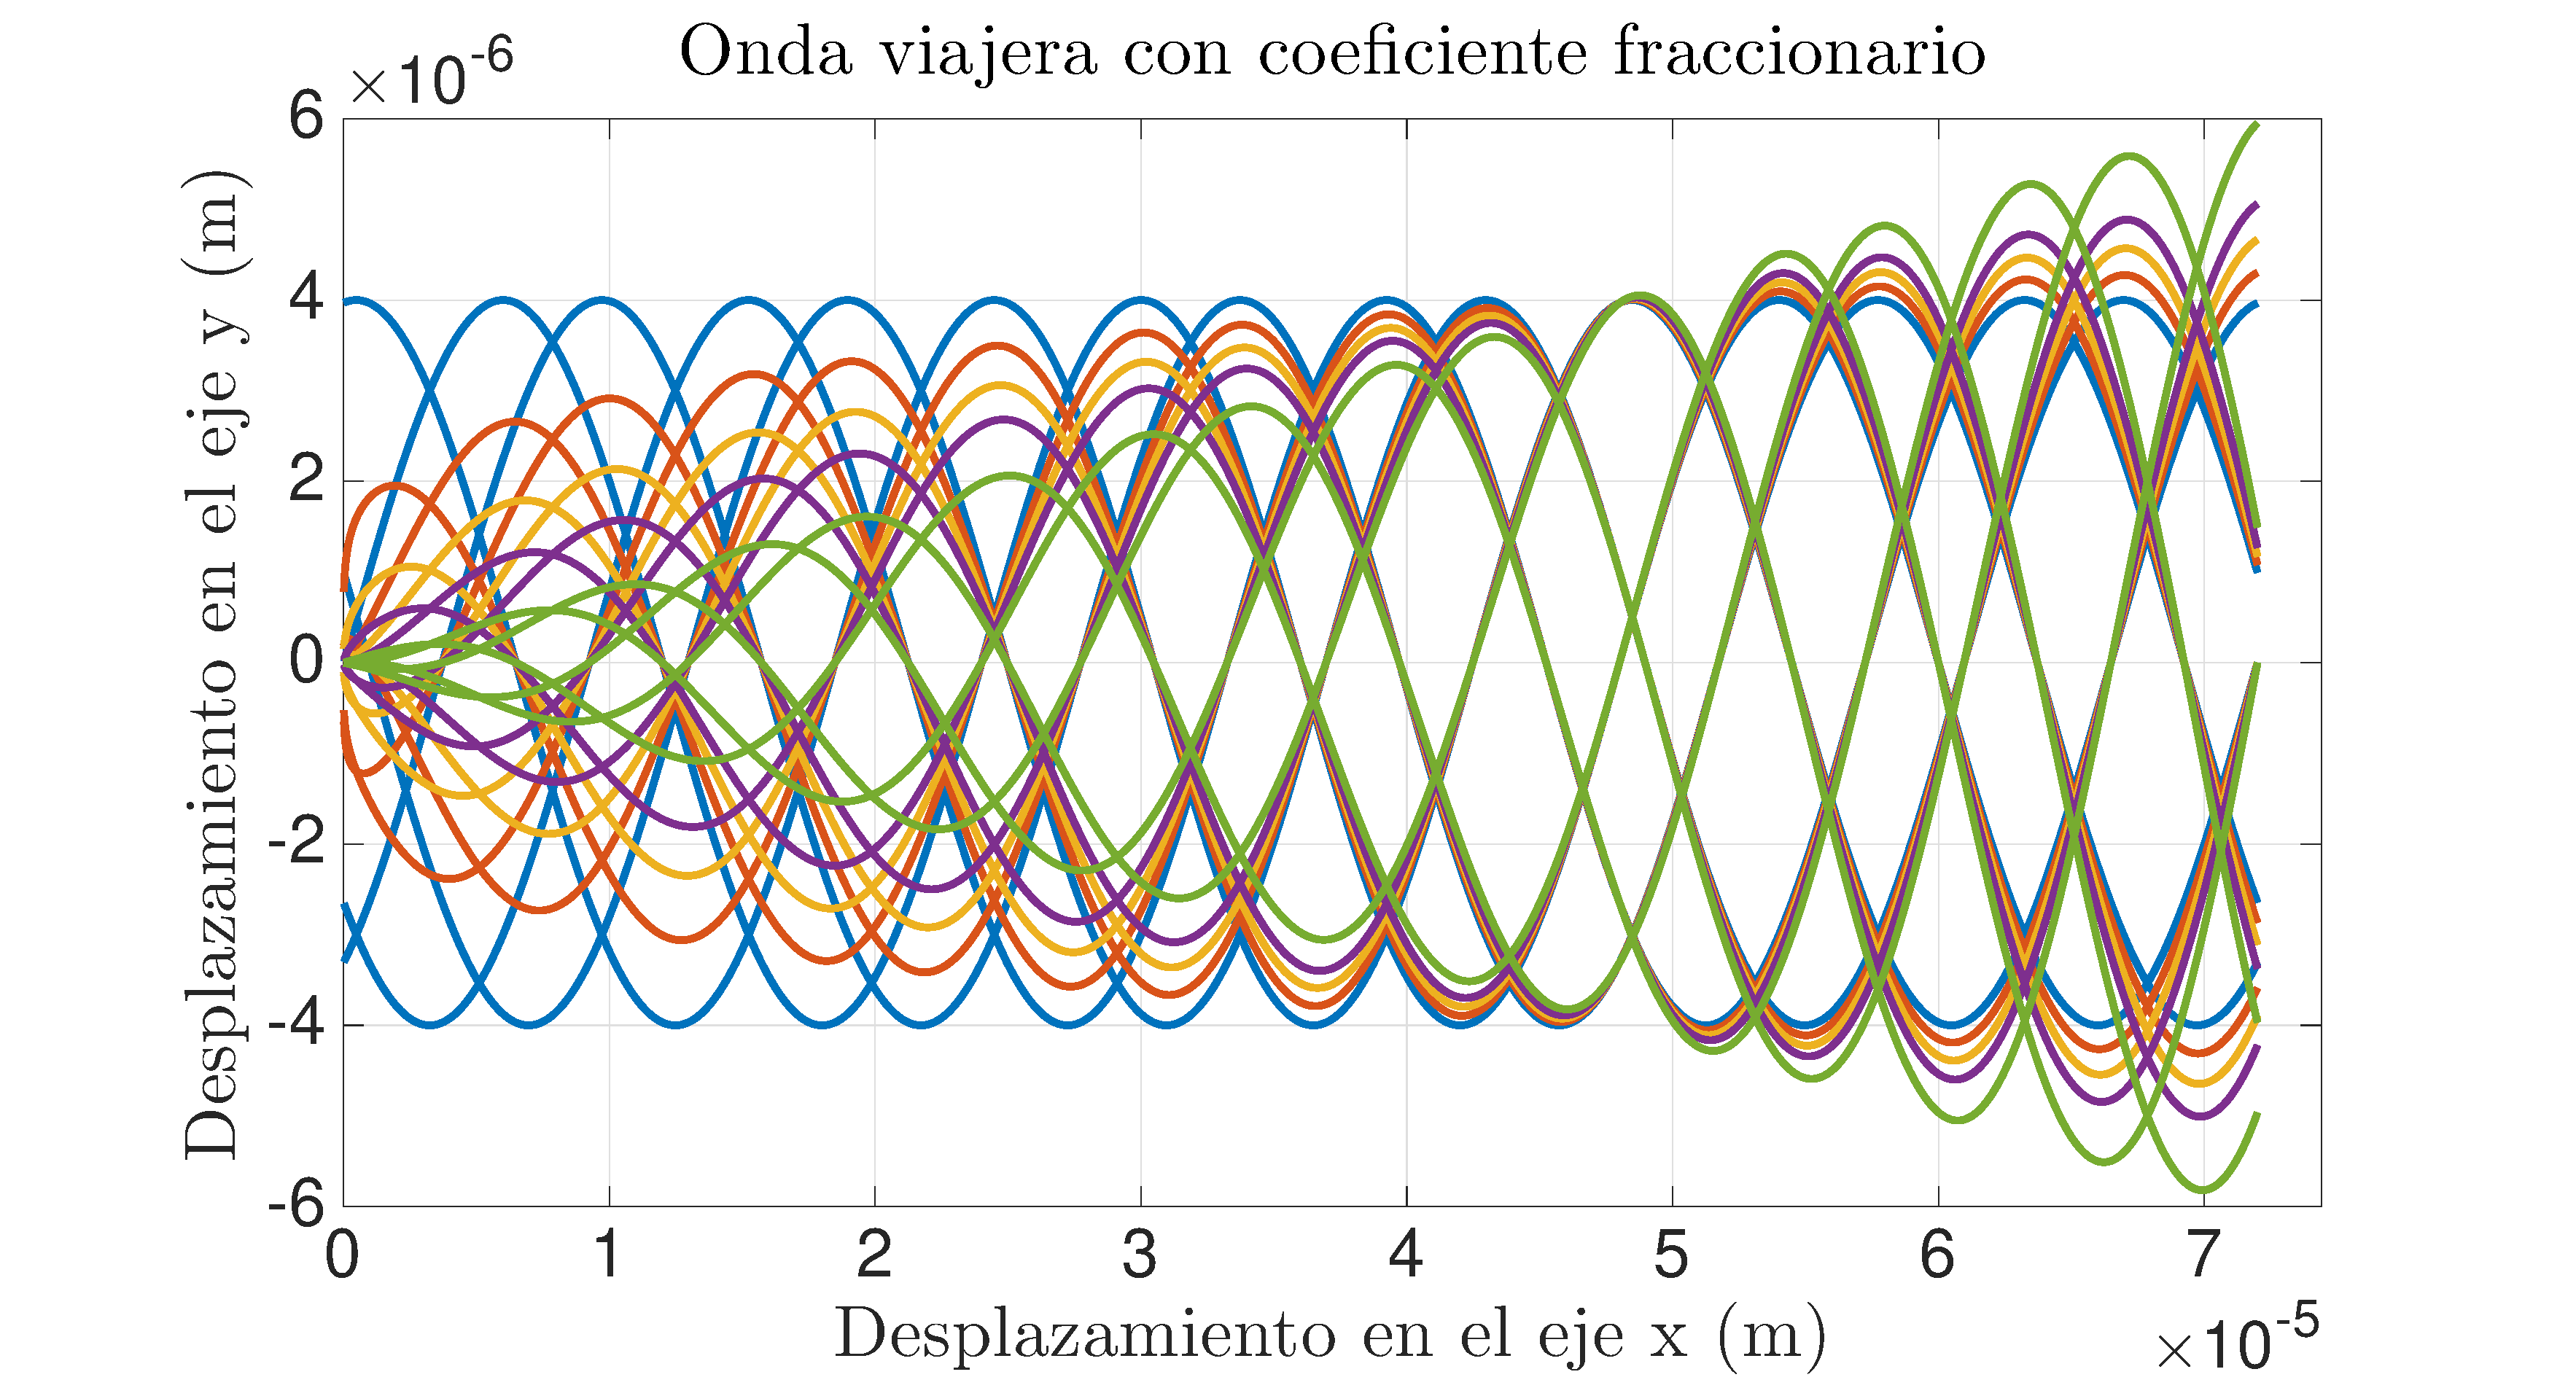
\includegraphics[width=0.6\textwidth]{Figuras/OVF}
  	\caption{Comparación de la onda viajera para diferentes coeficientes fraccionarios.}
  	\label{fig:OVF}
\end{figure}
 En esta representación el coeficiente $c_1$ es definido como $c_1 = \frac{A}{\lambda^{\alpha_0}}$, donde $A$ es la amplitud máxima de la oscilación, $\lambda$ la longitud del flagelo y $\alpha_0$ es $\alpha$, aunque valores próximos a este último permite modificar el crecimiento respecto a ese comportamiento fijo, pudiendo lograr crecimientos mas abrupto o suaves de las oscilaciones, si el valor es mayor o inferior respectivamente.\\
 
La onda de color azul representa el movimiento armónico de la onda viajera, mientras que las diferentes tonalidades, desde el color naranja hasta el verde representan el movimiento descrito para los valores de 0.2, 0.4, 0.6 y 1 de $\alpha$, respectivamente. Este barrido de valores de $\alpha$ permite determinar que valores cercanos a cero implican un crecimiento más rápido al inicio del flagelo y un crecimiento mas amortiguado una vez alcanzada la amplitud máxima deseada de las oscilaciones. Así mismo, valores próximos a la unidad implican un comportamiento completamente opuesto.\\

Mediante esta nueva expresión se consigue de definir un movimiento de onda viajera, cuyo crecimiento y modulación se encuentra regulado con un único parámetro. Además de proporcionar una velocidad mayor respecto al movimiento descrito en (\ref{eq:flag_fish_traveling_wave}) y por lo tanto más optima respecto al movimiento armónico de onda viajera. Aunque esta conclusión desea ser validada en este documento, en una primera instancia puede ser aceptada, pues a un 20.08\% de longitud del flagelo (10$^{-5}$ m ) el movimiento descrito por (\ref{eq:flag_fish_traveling_wave_fractional}) logra alcanzar una 73.12\% de la amplitud máxima deseada, frente al 21.06\% del movimiento representado por (\ref{eq:flag_fish_traveling_wave}).\\

Para justificar que este incremente de amplitud, se corresponde con un aumento de la fuerza de empuje y por lo tanto de la velocidad de avance, simplemente es necesario repetir el procedimiento que permitió calcular la velocidad de (\ref{eq:flag_fish_traveling_wave}) en (\ref{eq:Vx_fish}) \cite{gray1955propulsion}. Sin embargo, la integración del término exponencial de (\ref{eq:flag_fish_traveling_wave_fractional}) implica un proceso iterativo de resolución compleja. Inconveniente que pretende ser solventado mediante el uso de técnicas de integración numérica basado en una cuadratura adaptativa de Gauss-Kronrod.\\

A continuación se describe el procedimiento y software desarrollado para el calculado de la velocidad considerando oscilaciones de pequeña amplitud, donde los términos segundo orden son despreciados, y en una segunda perspectiva en la cual se tiene la influencia de dichos términos.



